\subsubsection{Transactions Set}

\begin{comment}
\begin{itemize}
  \item[-] transaction\_id: Unique identifier for each transaction in the database.
  \item[-] transaction\_start: Datetime when the transaction started. Format: DD/MM/YYYY HH:MM (ex. 1/1/2022 4:50).
  \item[-] transaction\_end: Datetime when the transaction was completed. Format: DD/MM/YYYY HH:MM (ex. 1/1/2022 4:54).
  \item[-] transaction\_amount: Amount of money involved in the transaction.
\end{itemize}

\begin{figure}[H]
    \centering
    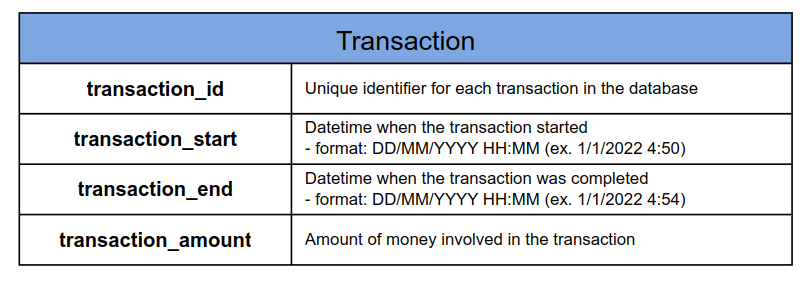
\includegraphics[scale = 0.40]{images/transaction.png}
    \caption{Transaction relation attributes}
    \label{img:pg-stable}
\end{figure}

\end{comment}

The transaction set constitutes the simulated input data stream continuously arriving to the system. Each transaction represents the operation done by a client's card on a ATM of the bank network. Therefore it has the form of a \emph{interaction} edge/relation from the volatile subgraph (see \ref{section:volatile-pg}) matching one Card with one ATM from the stable bank database.

Note that, as in our definition of the input data stream of the $DP_{CQE}$, we will generate two edges per transaction -- the \emph{opening} and the \emph{closing} edge -- which both will constitute a single \emph{interaction} relation. The \emph{opening} edge (Figure \ref{img:opening-edge}) will be the indicator of the begining of a new transaction between the matched Card and ATM, it contains the values of the properties related with the starting time \texttt{start}, the transaction \texttt{type} as well as the \texttt{id}. The \emph{closing} edge (Figure \ref{img:closing-edge}) will indicate the end of the transaction, completing the values of the rest of the properties of the \emph{interaction}: \texttt{end} and \texttt{amount}.


\begin{figure}[h]
  \centering
  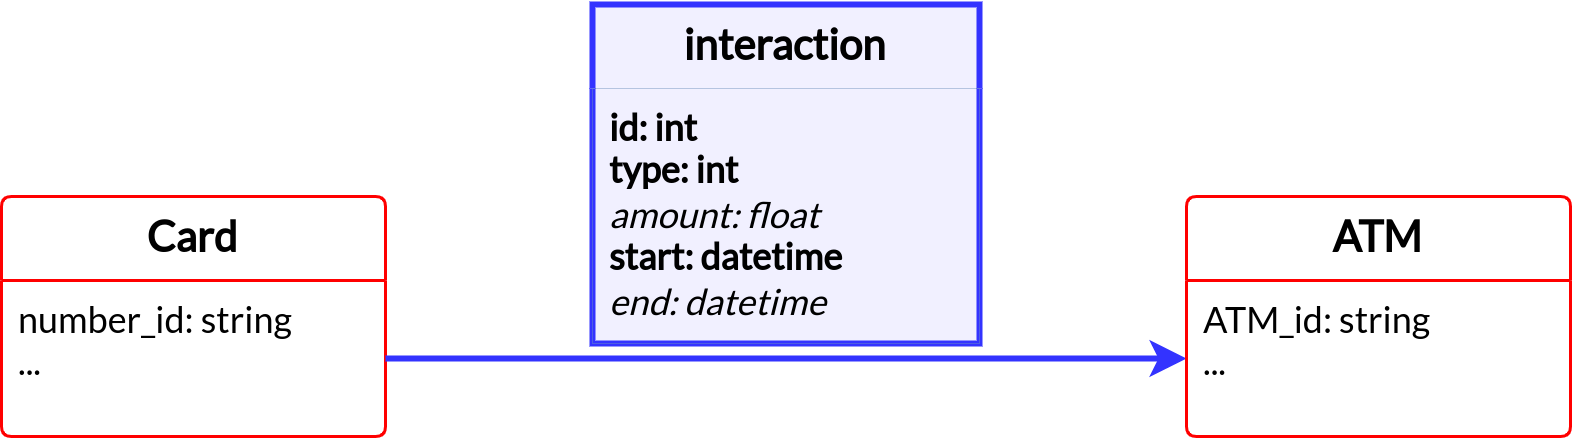
\includegraphics[scale = 0.8]{images/2-edges-tx-tfm.png}
  \caption{\emph{Opening} interaction edge}
  \label{img:opening-edge}
\end{figure}

\begin{figure}[h]
  \centering
  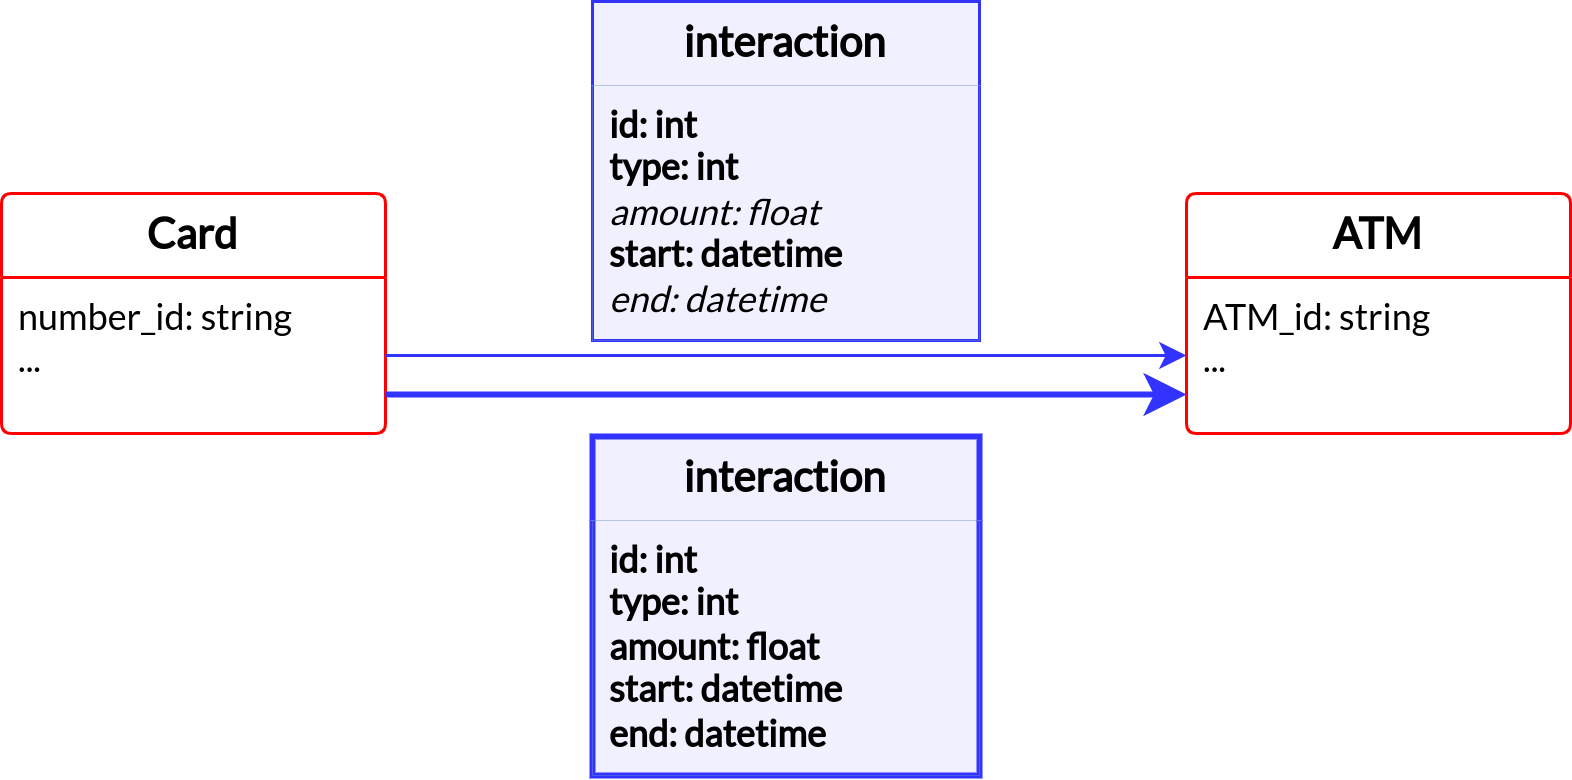
\includegraphics[scale = 0.8]{images/2-edges-tx-tfm-1.png}
  \caption{\emph{Closing} interaction edge}
  \label{img:closing-edge}
\end{figure}

We divide the generation of the transaction set in two subsets: the regular transaction set and the anomalous transaction set. The regular transaction set consists of the \emph{ordinary/correct} transactions, whereas the anomalous transaction set is composed of the \emph{irregular/anomalous} transactions that are intentionally created to produce anomalous scenarios.
The main objective under this division is the ability to have the control on the exact number of anomalous ATM transactions that we generate so that we can later measure the efficiency of our system detecting them. \textcolor{gray}{as we have the exact number of anomalous transactions created to compare with, represented by size of the anomalous subset. Otherwise, if we were generating all the transactions together at the same time it would be more difficult to have the control on the amount of anomalous scenarios created, so that later, it will not be possible to measure the efficiency of our system detecting them, since we will not know their amount.}


\textcolor{blue}{To do the generation of the synthetic set of transactions we created the Python program \texttt{transactionGenerator.py}. On it we need to specify the value of the parameters needed to customise the generation of the set of transactions.}

\textcolor{red}{TODO: DEFINE HOW TO RUN IT AND WHICH ARE THE PARAMETERS THAT WE NEED TO INTRODUCE}.

\paragraph{Regular Transaction Set\\}

\begin{tcolorbox}
  \begin{itemize}
    \item \textcolor{green}{$\Rightarrow$}\textbf{By card}: Generation of the transactions for each of the cards independently. \textbf{We have
    control} to avoid anomalous scenarios when selecting the ATMs and distributing the transactions along time.
    \item \textbf{In general}: Linking ATM and client composing (card,ATM) pairs, and distributing these pairs along
    time according to a certain distribution. \textbf{No control / More difficult to control the possible derived
    anomalous scenarios produced among same card pairs}.
  \end{itemize}
\end{tcolorbox}

Therefore, the generation by card option it is considered to be the best so to be able to have the control
on the possible anomalous scenarios for the generated transactions of each of the cards. Some ideas to explore:

\begin{itemize}
  \item Selection of ATMs:
  \begin{itemize}
    \item \textcolor{green}{$\Rightarrow$} Neighborhood / Closed ATM subset.
    \item Random walk. To do the selection of the sequence of ATMs for the generated transactions.
  \end{itemize}
  \item Distribution of the transactions along time:
  \begin{itemize}
    \item \textcolor{green}{$\Rightarrow$} Uniform distribution.
    \item \textcolor{blue}{$\Rightarrow$ (Consider the possibility)} Poisson process distribution.
  \end{itemize}
  \item Other options:
  \begin{itemize}
    \item Random walk for both the ATM and the transaction time selection, in the same algorithm together.
  \end{itemize}
\end{itemize}

\textcolor{red}{TODOS:
\begin{itemize}
\item Cambiar/Actualizar dibujos
\item Poner lista de params y explicar (tabla) como y qué se puede configurar
\item Prerequisitos: csv directory has to exist - create it beforehand better
\item Output files that are generated: regular, anomalous and all csvs.
\item Anomalous generator:
\begin{itemize}
  \item NO-Overlapping assumption - Explain
  \item Any type of tx to produce the fraud -> does not matter the type for the FP1.
\end{itemize}
\end{itemize}
}

The key idea of the transactions of this set is to avoid the creation of anomalous scenarios among them, so to have a close-to-reality simulation of a bank transaction stream flow free of anomalies. After this set is created, the transactions producing anomalous scenarios related with each specific fraud pattern will be produced.


We generate transactions for each of the generated cards on our bank network, based on each of the gathered card transaction behavior. The regular transaction data stream is generated for a customisable \texttt{NUM\_DAYS} number of days starting in a \texttt{START\_DATE}. On what follows we give the details on the procedure done for each of the cards:

\textcolor{gray}{
For a card, the idea is to create a certain 
number of transactions per day, by linking the card to a certain ATM that is no farther 
than \textcolor{orange}{\texttt{max\_distance}} kms from the residence location of the 
client of the card. Also, we will limit the time distance between two consecutive 
transactions so that the final set of created transactions can not produce a potential 
fraud related with having two transactions in different ATM locations with an insufficient 
feasible time distance.
}

\begin{enumerate}
    \item \textbf{Creation of the ATM subset}: Among all the ATMs of the stable bank database we create a subset of ATMs, such that all the regular transactions generated for this card take place in (randomly selected) ATMs of this subset. 
    \textcolor{red}{TODO: ALIGN THIS}
    $$\texttt{ATM\_subset} = \{\texttt{ATM}\ \\
    |\ \texttt{distance(ATM,residence\_loc)} \leq \texttt{MAX\_DISTANCE\_SUBSET\_THRESHOLD}\}$$

    \texttt{ATM\_subset} consists of the ATMs that are considered to be \textit{usual} for the card, considering the ATMs that are at a distance lower or equal to a customisable maximum distance threshold \texttt{MAX\_DISTANCE\_SUBSET\_THRESHOLD} to the registered residence location \texttt{residence\_loc} on the card. We also limit the size of this subset, considering only a maximum ratio of the total number of ATMs (\texttt{MAX\_SIZE\_ATM\_SUBSET\_RATIO} $\in [0,1]$), so that only a certain ratio of the closest ATMs are included on it.

    $$|\texttt{ATM\_subset}| = \texttt{MAX\_SIZE\_ATM\_SUBSET\_RATIO} * |\texttt{ATM}|$$

\textcolor{red}{TODO: CAMBIAR ESTA IMAGEN}
    \begin{figure}[H]
      \centering
      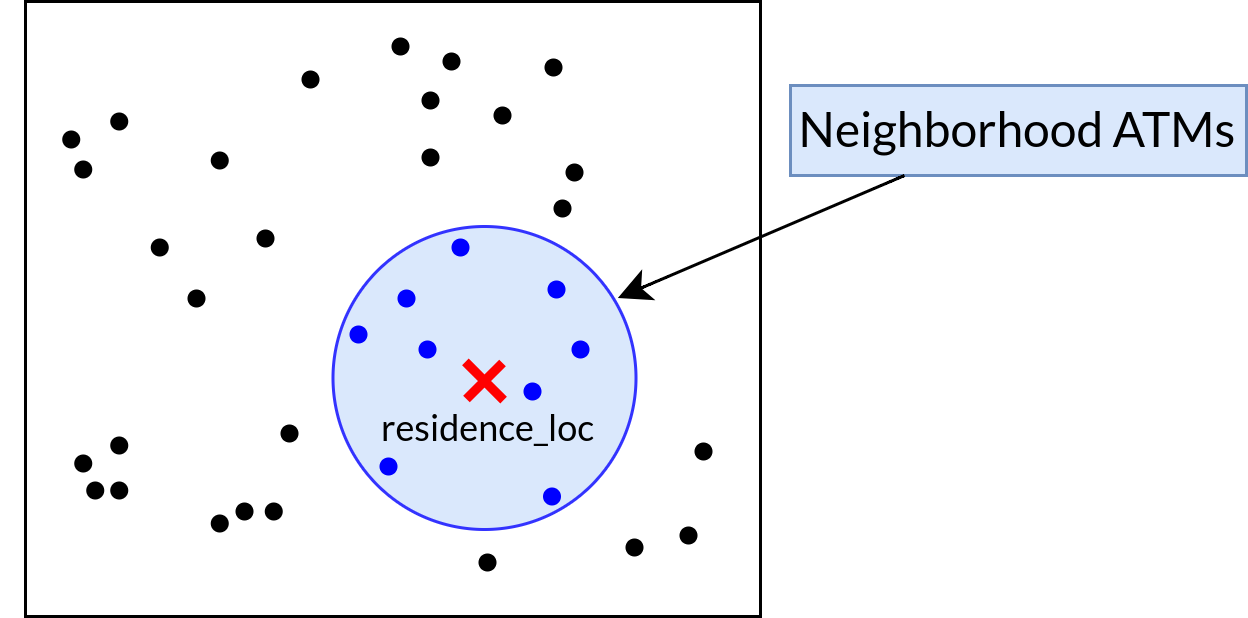
\includegraphics[scale=1.1]{images/tx-generation-1-named.png}
      \caption{\texttt{Neighborhood} ATM subset}
    \end{figure}

    \item \textbf{Calculate \texttt{t\_min\_subset}}: Minimum threshold time between any two consecutive transactions of the card. That is, the minimum time distance between the end of a transaction and the start of the next consecutive transaction of a card. For it, we take the time needed to traverse the maximum distance between any pair of ATMs of the \texttt{ATM\_subset}: \texttt{max\_distance\_subset} at an assumed speed that any two points can be traveled for the case of ordinary scenarios: \texttt{REGULAR\_SPEED}.
    $$\texttt{t\_min\_subset} = \frac{\texttt{max\_distance\_subset}}{\texttt{REGULAR\_SPEED}}$$

    \item \textbf{Decide the number of transactions \texttt{num\_tx}}:
    Based on the behavior of the card, we decide the number of transactions (\texttt{num\_tx}) to generate for the card for the selected number of days \texttt{NUM\_DAYS} as:

    $$\texttt{num\_tx} \sim \text{Poisson}(\lambda = \texttt{ops\_day} * \texttt{NUM\_DAYS})$$ where \texttt{ops\_day} is the sum of the average number of all the kinds of operations per day of the particular card: 
    $$\texttt{ops\_day} = \texttt{withdrawal\_day} + \texttt{ deposit\_day} + \texttt{ inquiry\_day} + \texttt{ transfer\_day}$$


    \item \textbf{Decide on the type of transaction}: for each of the \texttt{num\_tx} transactions, the transaction \texttt{type} is decided randomly assigning a transaction \texttt{type} given a probability distribution constructed from the card behavior:
    
    $$
    \begin{cases}
      P(\texttt{type} =  \texttt{withdrawal}) = \frac{\texttt{withdrawal\_day}}{\texttt{ops\_day}} \\[8pt]
      P(\texttt{type} =  \texttt{deposit}) = \frac{\texttt{deposit\_day}}{\texttt{ops\_day}} \\[8pt]
      P(\texttt{type} = \texttt{inquiry}) = \frac{\texttt{inquiry\_day}}{\texttt{ops\_day}} \\[8pt]
      P(\texttt{type} =  \texttt{transfer}) = \frac{\texttt{transfer\_day}}{\texttt{ops\_day}} 
    \end{cases}
    $$

    \item \textbf{Distribution of the \texttt{num\_tx} transaction times}: along the selected number of days \texttt{NUM\_DAYS} time interval.
    
    We do a random uniform distribution of the \texttt{num\_tx} transaction times
    in the time interval starting in \texttt{START\_DATE} and finishing \texttt{NUM\_DAYS} days after, obtaining the \texttt{start} and \texttt{end} times for each of the \texttt{num\_tx} transactions, with the constraint that, for each transaction $i$, the next one $i+1$ is at a minimum time distance of \texttt{t\_min\_subset}. Specifically, the transaction times are generated guaranteeing:

    $$i.\texttt{end} + \texttt{t\_min\_subset} < (i+1).\texttt{start} \ \forall i \in [1,\texttt{num\_tx})$$

    The \texttt{end} time of a transaction is assigned a shifted time difference with respect to the \texttt{start} time. In particular:

    $$
    \texttt{end} = \texttt{start} + \texttt{time\_difference}
    $$

    where:

    $$\texttt{time\_difference} \sim \mathcal{N}(\texttt{MEAN\_DURATION},\,\texttt{STD\_DURATION})$$ with the corrections:

    $$
    \texttt{time\_difference} =
    \begin{cases} 
        \texttt{MEAN\_DURATION} & \text{if } \texttt{time\_difference} < 0 \\
        \texttt{MAX\_DURATION} & \text{if } \texttt{time\_difference} > \texttt{MAX\_DURATION} \\
        \texttt{time\_difference} & \text{otherwise}
    \end{cases}
    $$

\textcolor{red}{TODO: PONER UN DIBUJITO!, explicar lo del checking de los fitting holes? --> yo creo que esto ya no es necesario... demasiado detalle}


  \item Assign a transaction \texttt{amount}: assigned depending on the \texttt{type} based on card behavior:
    
  $$
  \begin{cases}
    \mathcal{N}(\texttt{amount\_avg\_withdrawal},\, \texttt{amount\_std\_withdrawal}) & \text{if } \texttt{type} = \texttt{withdrawal} \\[10pt]
    
    \mathcal{N}(\texttt{amount\_avg\_deposit},\, \texttt{amount\_std\_deposit}) & \text{if } \texttt{type} = \texttt{deposit} \\[10pt]

    0 & \text{if } \texttt{type} = \texttt{inquiry} \\[10pt]
    
    \mathcal{N}(\texttt{amount\_avg\_deposit},\, \texttt{amount\_std\_transfer}) & \text{if } \texttt{type} = \texttt{transfer}
  \end{cases}
  $$

  $$
  \text{If } \texttt{amount} < 0, \text{ then re-draw from } U(0, 2 \cdot \texttt{amount\_avg\_type}).
  $$

  with \texttt{amount\_avg\_type} as \texttt{amount\_avg\_withdrawal}, \texttt{amount\_avg\_deposit} or \texttt{amount\_avg\_deposit} depending on the respective transaction \texttt{type}.

\end{enumerate}

As a summary we show a pseudocode of the transaction generator in Algorithm \ref{alg:regular-tx-generator}.

\begin{algorithm}[H]
  \small
  \begin{algorithmic}[1]
  \STATE $\texttt{id} \gets 0$
  \FOR{\text{card} in \text{cards}}
    \STATE $\texttt{ATM\_subset}, \overline{\texttt{ATM\_subset}} \gets \text{createATMsubset(\texttt{residence\_loc})}$
    \STATE $\texttt{t\_min\_subset} \gets \text{calculate\_t\_min\_subset(\texttt{ATM\_subset})}$
    \STATE $\texttt{num\_tx} \gets \text{decide\_num\_tx()}$
    \STATE $T \gets \text{distribute}(\texttt{num\_tx}, \texttt{t\_min\_subset})$
    \FOR{$t_i$ in $T$}
        \STATE $\texttt{ATM}_{i} \sim \texttt{ATM\_subset}$
        \STATE $\texttt{start}_{i} \gets t_i.start$
        \STATE $\texttt{end}_{i} \gets t_i.end$
        \STATE $\texttt{type}_{i} \gets \text{getType()}$
        \STATE $\texttt{amount}_{i} \gets \text{getAmount()}$
        \STATE $\texttt{id}_{i} \gets \texttt{id}; \ \texttt{id} \gets \texttt{id} + 1$
        \STATE $\text{createTransaction}(\texttt{id}_{i}, \texttt{ATM}_i, \texttt{start}_{i},\texttt{end}_{i}, \texttt{type}_{i}, \texttt{amount}_i)$
    \ENDFOR
    \STATE $\text{introduceAnomalous}(\texttt{ATM\_subset}, \overline{\texttt{ATM\_subset}})$
  \ENDFOR
  \end{algorithmic}
  \caption{Regular Transactions Generation}
  \label{alg:regular-tx-generator}
\end{algorithm}

\textcolor{red}{TODO: PONER NOMBRES DE LAS FUNCIONES EMPLEADAS - REFERENCIAS EN EL TEXTO DE LA EXPLICACIÓN DE ARRIBA!}

\paragraph{Anomalous Transaction Set\\}

After the generation of regular transactions we perform an injection of transactions to produce anomalous scenarios. The injection is taylored depending on the specific kind of 
anomalous scenarios that we want to produce. In what follows we explain the injection process depending on each of the types of frauds that we have considered.

\paragraph{Fraud Pattern I}

To produce anomalous scenarios related to this type of fraud, we produce the injection
of transactions that will produce the satisfaction of this fraud pattern. In other words,
we inject transactions that violate the minimum \emph{time-distance} constraint between transactions performed with the same card. Therefore, as we can see in Figure \ref{img:anomalous-type-1}, if we consider a set of regular transacions for a certain card, where $y_1$ and $y_2$ are regular consecutive transactions, we will introduce an anomalous transaction $a_{12}$ such that: 

$$(y_1.\texttt{ATM\_id} \ne a_{12}.\texttt{ATM\_id}) \land (a_{12}.\texttt{start} - 
y_1.\texttt{end} < T_{min}(y_1.\texttt{ATM\_loc}, a_{12}.\texttt{ATM\_loc}))$$

where \texttt{ATM\_loc} is the tuple of coordinates (loc\_latitude,loc\_longitude) of the corresponding ATM. This injection will produce an anomalous scenario of this kind of fraud with at least the $y_1$ previous transaction. Note that, it could possibly trigger more anomalous fraud scenarios with the subsequent transactions ($y_2$ and on...).

\begin{figure}[H]
    \centering
    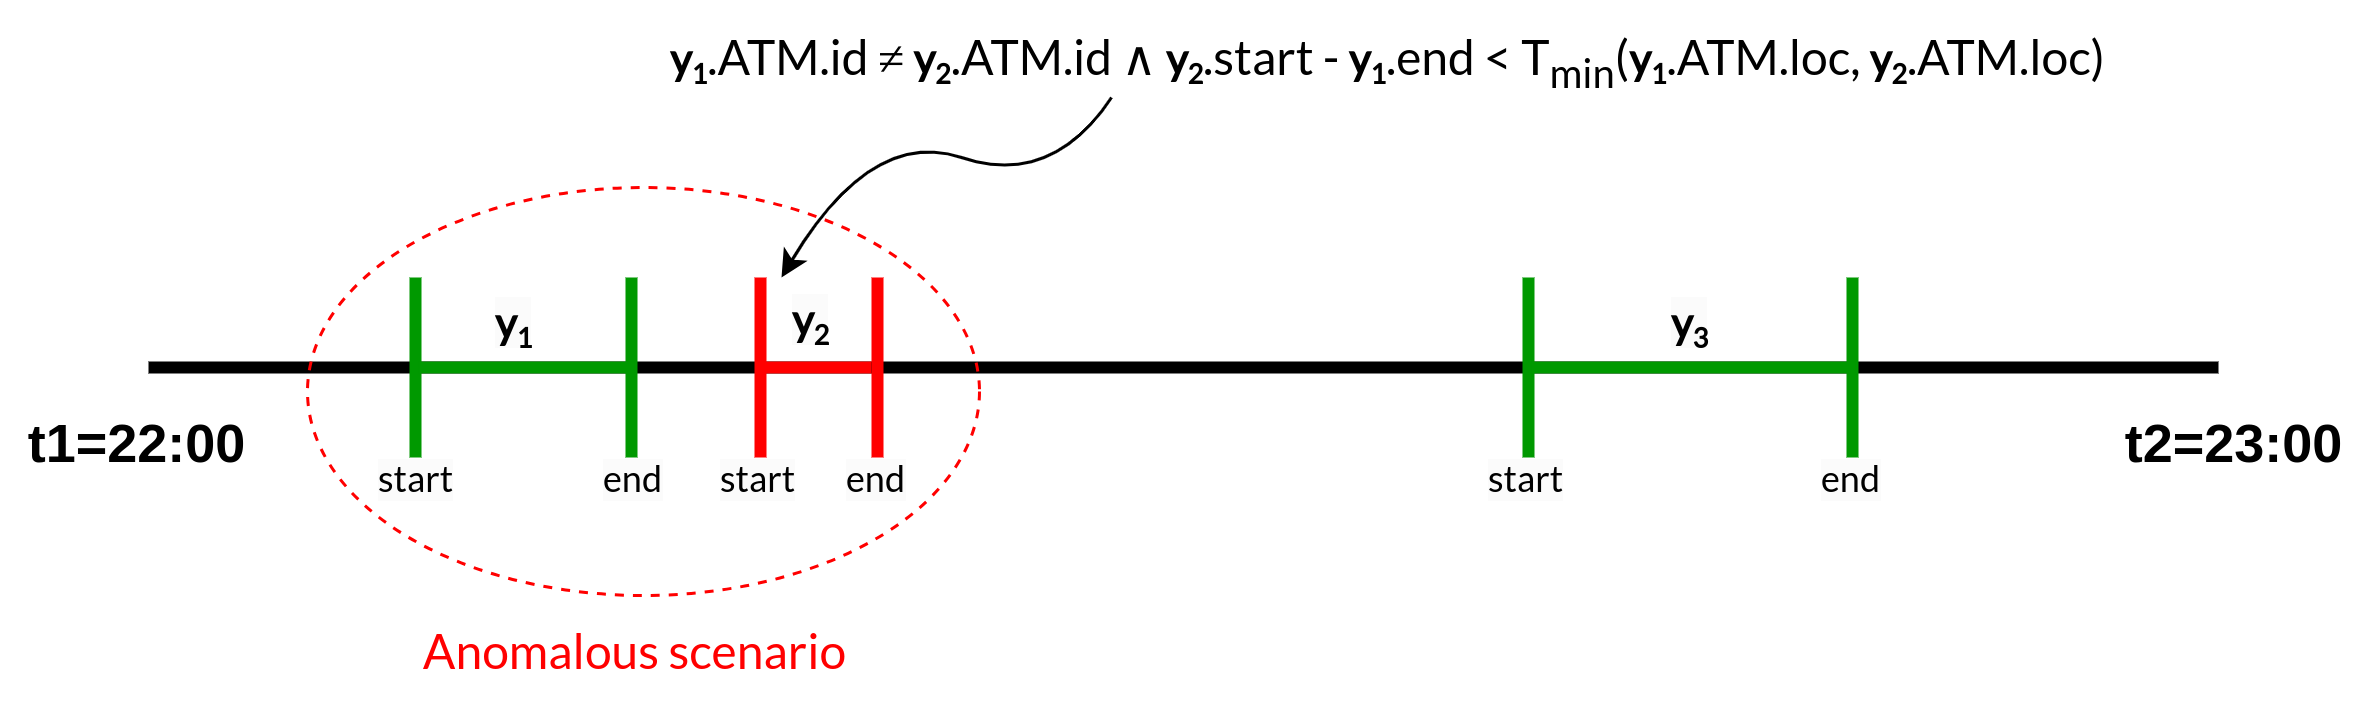
\includegraphics[width=\textwidth]{images/tx-generation.png}
    \caption{Creation of anomalous scenario - type I}
    \label{img:anomalous-type-1}
\end{figure}

Some assumptions related with the generation of anomalous transactions for this kind of fraud pattern are:
\begin{itemize}
  \item \textbf{Overlapping of transactions is not possible}:
  Appart from guaranteeing that this injection causes at least one anomalous scenario, we also respect the additional constraint of ensuring that the anomalous transaction injected does not cause overlapping with any of the transactions, in particular neither with the previous nor the next one. \textcolor{orange}{This constraint is added based on the assumption that the bank itself does not allow to open a transaction whenever another one is still open.} Therefore considering that $a_{12}$ is the anomalous injected transaction in between the regular consecutive transactions $y_1$ and $y_2$, when generating $a_{12}$ we guarantee that:
  $$
  \begin{cases}
    a_{12}.\texttt{start} > y_{1}.\texttt{end} \\
    a_{12}.\texttt{end} < y_{2}.\texttt{start}
  \end{cases}
  $$
  \item \textbf{There are no two consecutive anomalous transactions}: For simplicity in our practical purposes, we do the generation of anomalous transactions for this kind of fraud pattern assuming that an anomalous transaction can only be in between two regular consecutive transactions, so that we do not consider the case of the injection of two or more consecutive anomalous transactions for this kind of fraud. See Figure \ref{img:anomalous-type-1-insertion-points}.
  \begin{figure}[H]
    \centering
    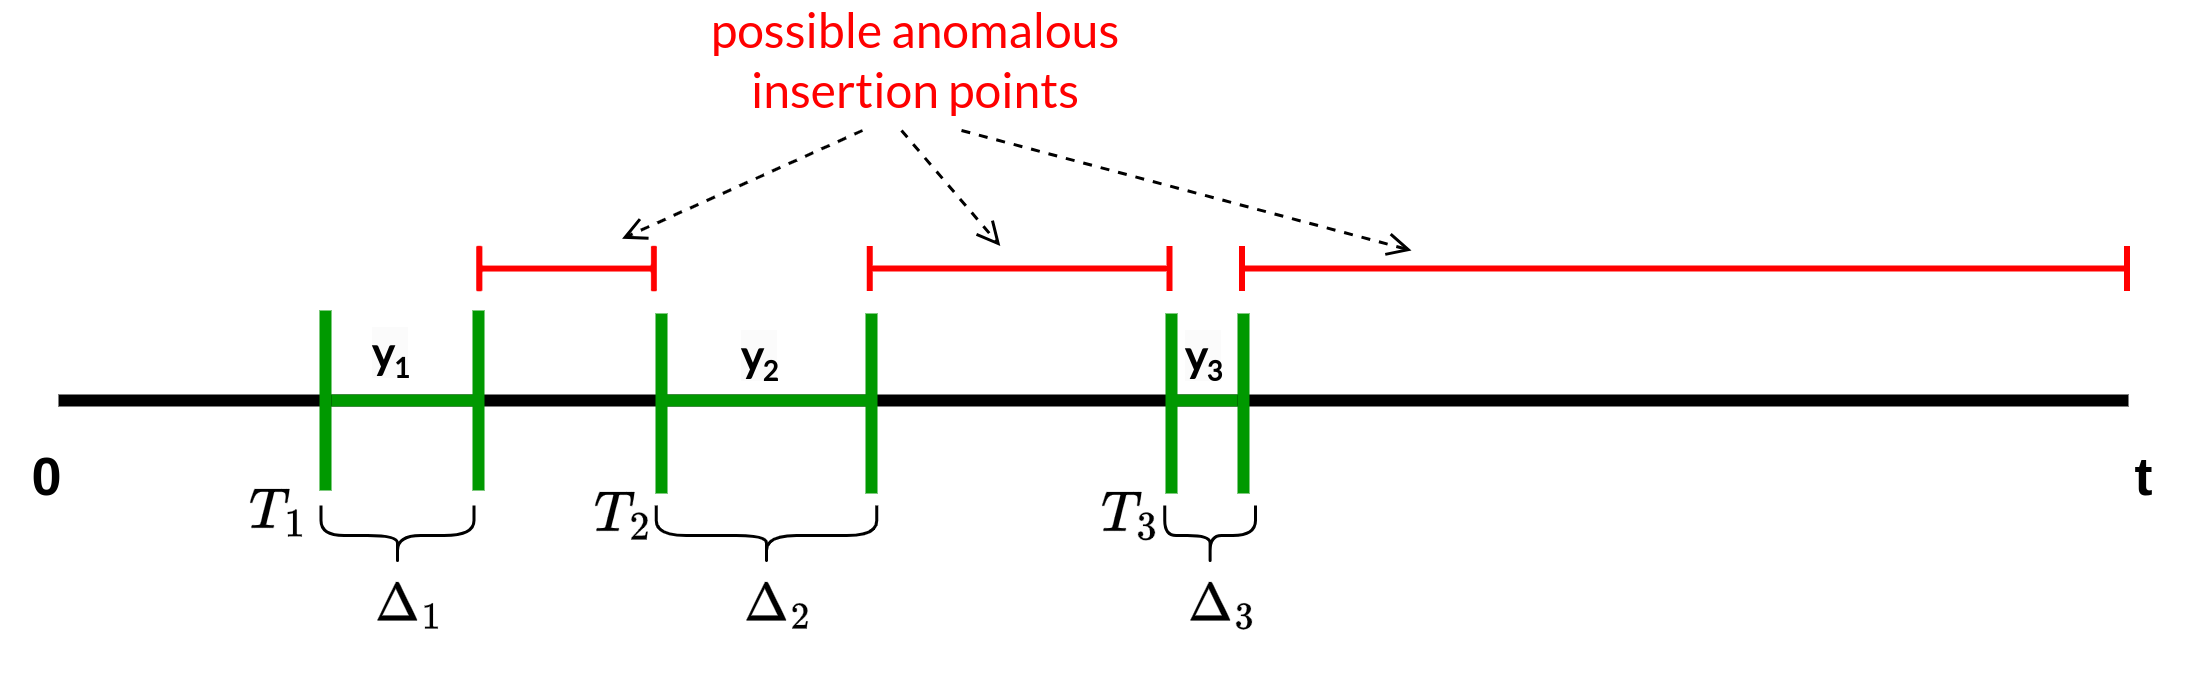
\includegraphics[width=\textwidth]{images/tx-generation-anomalous-1.png}
    \caption{Considered possible injection points of anomalous transactions of fraud type I}
    \label{img:anomalous-type-1-insertion-points}
  \end{figure}  
\end{itemize}

We generate $\texttt{ANOMALOUS\_RATIO\_1} * \texttt{num\_tx}$ anomalous transactions for each of the cards related with the fraud pattern I, where $\texttt{ANOMALOUS\_RATIO\_1} \in [0,1]$ defines the ratio of anomalous transactions of this kind over the total number of regular transactions \texttt{num\_tx} for each of the cards. In Algorithm \ref{alg:anomalous-tx-generator-1} we describe at a high level the process of the generation of anomalous transactions for this kind of fraud pattern. 


\textcolor{red}{Preconditions:
\begin{itemize}
  \item ATMsubset, and the compl. are given by param, from the tx regular generator
\end{itemize}
}

\begin{algorithm}[H]
  \small
  $\textbf{introduceAnomalous}(\texttt{ATM\_subset}, \overline{\texttt{ATM\_subset}})$
  \begin{algorithmic}[1]
  \STATE $\texttt{num\_anomalous} \gets \texttt{num\_tx} * \texttt{ANOMALOUS\_RATIO\_1}$
  \STATE $i \gets 0$
  \WHILE{$i < \texttt{num\_anomalous}$}
      \STATE $\texttt{ATM}_{i} \sim \overline{\texttt{ATM\_subset}}$
      \STATE $prev_i, next_i \gets \text{randomUniquePosition(\texttt{num\_tx})}$
      \STATE $t_i \gets \text{getTime}(prev_i, next_i)$
      \STATE $\texttt{start}_{i} \gets t_i.start$
      \STATE $\texttt{end}_{i} \gets t_i.end$
      \STATE $\texttt{type}_{i} \gets \texttt{getRandomType()}$
      \STATE $\texttt{amount}_{i} \gets \texttt{getAmount()}$
      \STATE $\texttt{id}_{i} \gets \texttt{id}; \ \texttt{id} \gets \texttt{id} + 1$
      \STATE $\texttt{createTransaction}(\texttt{id}_{i}, \texttt{ATM}_i, \texttt{start}_{i},\texttt{end}_{i}, \texttt{type}_{i}, \texttt{amount}_i)$
      \STATE $i \gets i + 1$
  \ENDWHILE
  \end{algorithmic}
  \caption{Introduction of Anomalous Transactions for Fraud Pattern I}
  \label{alg:anomalous-tx-generator-1}
\end{algorithm}


\begin{enumerate}
  \item \textbf{Assignment of ATMs not belonging to the \texttt{ATM\_subset}}: the anomalous transactions are linked to ATMs that are part of the complementary of the \texttt{ATM\_subset}.
  \item \textbf{Each anomalous transaction has a unique insertion position}: As described previously, we do not allow the case of two or more consecutive anomalous transactions injection. Each anomalous transaction occupies a unique position among all the possible injection positions defined by the set of regular transactions generated for the card. As it can be seen on Figure \ref{img:anomalous-type-1-insertion-points}, considering that we have three regular transactions, we will consider three unique possible insertion points for the anomalous transactions. The procedure of assigning a unique insertion position for each anomalous transaction to be generated is achieved with the function \text{randomUniquePosition(\texttt{num\_tx})}, that given the number of regular transactions of the card \texttt{num\_tx} returns the previous and the next regular transaction to the assigned unique position.
  \item \textbf{Assign transaction times such that respecting the needed time constraints}: in particular there are two time constraints to be satisfied:
  \begin{itemize}
    \item Production of fraud pattern with prev\_i
    \item No overlapping with prev\_i nor with next\_i
  \end{itemize}
  This is summarized in the pseudocode as the procedure getTime(prev\_i, next\_i), which returns $t_i$, as the tuple of (\texttt{start},\texttt{end}) times.
  \item \textbf{Random transaction type}
  \item \textbf{Arbitrary amount}
 
\end{enumerate}


\textcolor{red}{TODO: MENCIONAR MÁS COSAS EN UN LISTADO, COMO EN LA GENERACIÓN DE TX REGULARES?!}

\begin{comment}
\subsubsection{ATM closed subset + Poisson Process}

\begin{tcolorbox}
  \begin{itemize}
    \item[$\rightarrow$] \textbf{ATM selection}: Closed ATM subset.
    \item[$\rightarrow$] \textbf{Time distribution}: Poisson process distribution of $num\_tx$ 
    transactions for each of the cards.
  \end{itemize}
\end{tcolorbox}

Generate $\texttt{num\_tx}$ transactions for a selected period of time $\texttt{t}$.
Distribution following a Poisson process distribution along $[0,t]$.
\begin{itemize}
    \item[$\bullet$] $\lambda=\texttt{avg\_tx}$ on a day for the client if $\texttt{t = 24h}$. Otherwise, 
    decide a specific $\lambda$ for the considered $\texttt{t}$.
    \item[$\bullet$] Inter-arrival times $X_1, X_2, \cdots$ are distributed following an exponential distribution:
    $X_i \sim \text{Exp}(\lambda)$. They represent the time elapsed between two of these events, e.g. $X_2$ represents the time elapsed between the first and the second arrival. Note that in this case, since we need to respect the minimum required time between two consecutive 
    transactions ($t_{min}$) so to avoid introducing anomalous undesired scenarios, we have to impose
    that: $X_i \geq \Delta_{i-1} + t_{min}, \forall X_i$, where:

    \begin{itemize}
      \item[$\circ$] $X_{i}$: time elapsed between the $i$-$1$ and $i$-th transaction.
      \item[$\circ$] $\Delta_{i-1}$: time duration of the $i$-$1$ transaction. This duration will 
      be upper bounded by $\Delta_{max}$, which will be considered the maximum possible duration of a transaction.
      \item[$\circ$] $t_{min}$: minimum calculated time distance between any 2 consecutive transactions of the client.
  \end{itemize}

    With these interarrival times, we obtain the arrival times $T_i$. Note that they are not independent, in particular:
    $T_1 \leq T_2 \leq T_3 \cdots$.

    Therefore, to generate the Poisson process with rate $\lambda$:
    \begin{enumerate}
      \item Generate i.i.d. random variables $X_1, X_2, \cdots$ where $X_i \sim \text{Exp}(\lambda)$.
      \item Obtain the arrival times as:
        \begin{itemize}
          \item $T_1 = X_1$
          \item $T_2 = X_1 + X_2$
          \item $T_3 = X_1 + X_2 + X_3$
          \item $\cdots$
        \end{itemize}
    \end{enumerate}

    Note that, having imposed the previous we will have that:
    \begin{equation}
      \begin{cases}
        T_i = T_{i-1} + X_i \\
        X_i \geq \Delta_{max} + t_{min}
      \end{cases}\forall X_i \
    \end{equation}

    which implies that:
    
    \begin{equation}
      T_i \geq T_{i-1} + \Delta_{max} + t_{min}, \forall X_i
    \end{equation}
    
\end{itemize}
\begin{figure}[H]
    \centering
    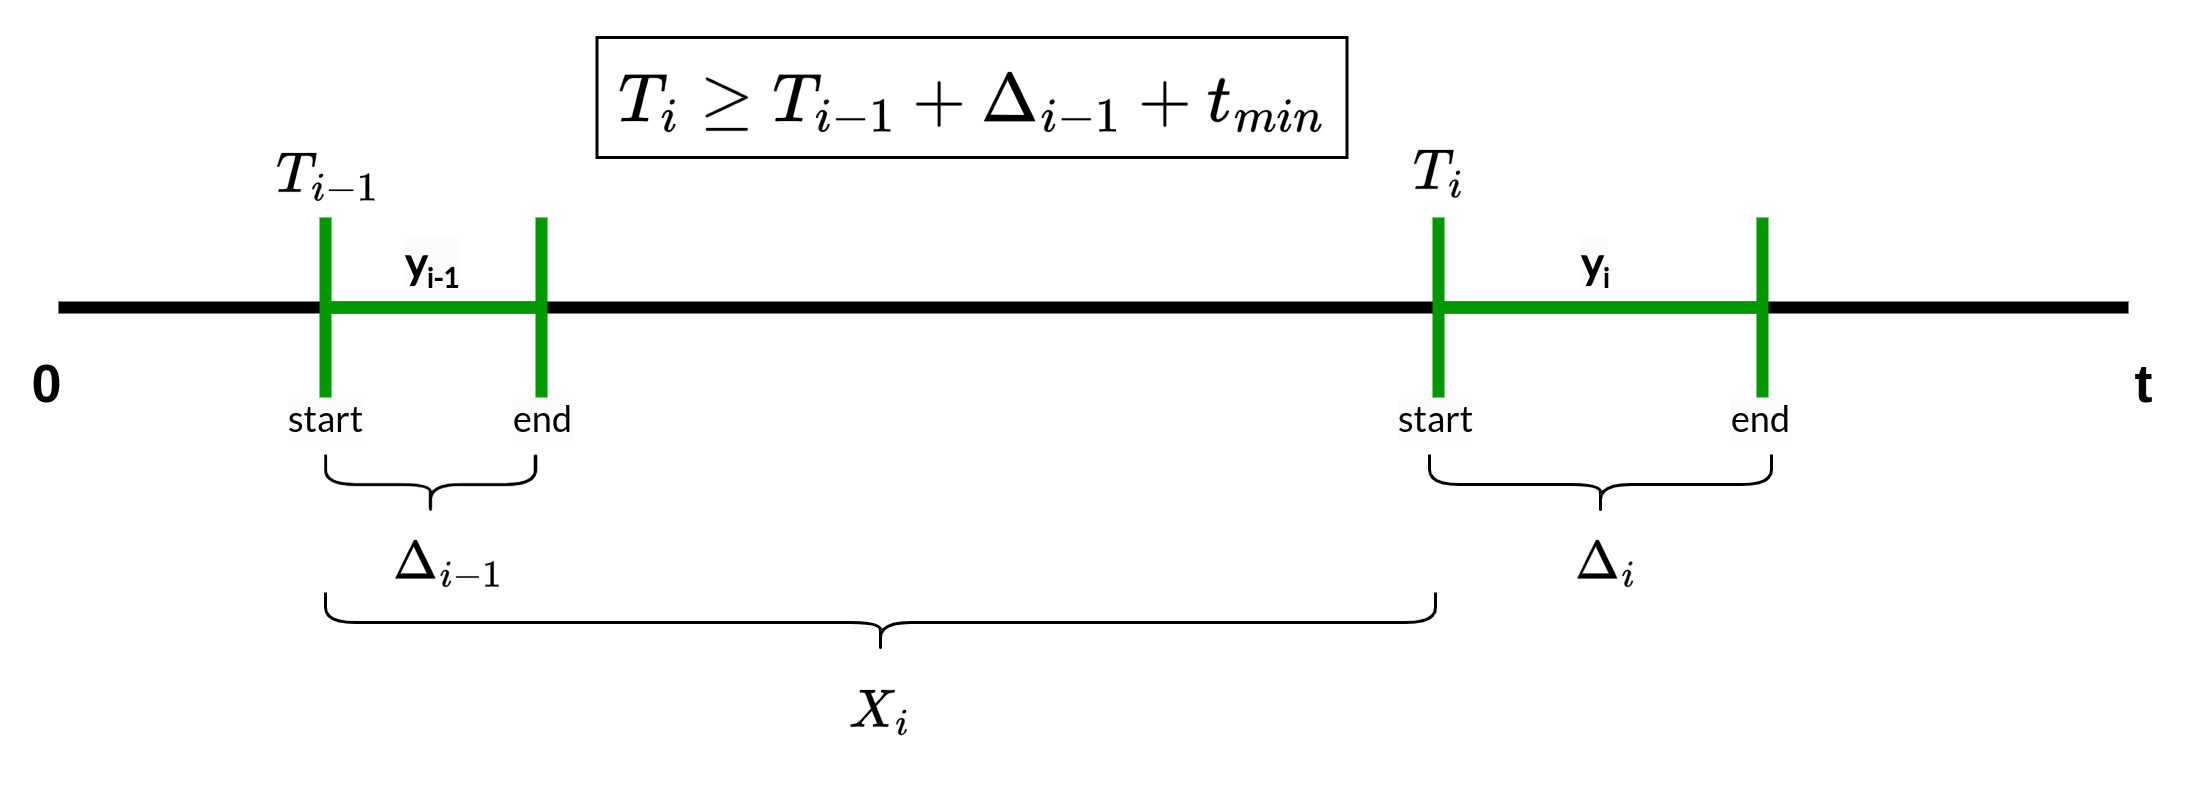
\includegraphics[scale=0.55]{images/tx-generation-dist-corrected.png}
    \caption{Schema of the interarrival and arrival event times on the poisson process.}
\end{figure}


References:

\begin{itemize}
  \item \href{https://www.probabilitycourse.com/chapter11/11_1_2_basic_concepts_of_the_poisson_process.php}{Poisson process modeling - Theoric description}
  \item \href{https://www.probabilitycourse.com/chapter14/Chapter_14.pdf}{Poisson process modeling - Python implementation}
  \item \href{https://timeseriesreasoning.com/contents/poisson-process/}{Less formal explanation with Python code}
  \item \href{https://www.math.wsu.edu/faculty/genz/416/lect/l05-45.pdf}{More theory}
  \item \href{https://en.wikipedia.org/wiki/Poisson_point_process}{Wikipedia entry}
\end{itemize}

\subsubsection{Random Walk / Markov Chain}

Idea is to model the sequence of transactions for each of the clients as a markov chain through the
network of ATMs. The network is a fully-connected graph with ATMs as nodes and edges are
weighted with the distance between each pair of ATMs as weights.

The idea is to obtain the sequence of transactions for each client as a markov chain, in which,
for each step a transaction is generated in that specific ATM node, at a certain datetime 
respecting the constraint of the minimum time distance with the previous transaction, so 
that no undesired anomalous fraud scenarios are produced. \\ 

Some considerations:
\begin{itemize}
  \item Initially, we will compute the transition matrix obtaining all the respective 
  transition probabilities. The probability of transition to another ATM-node will be 
  inversely proportional to the distance to the considered ATM-node.
  \item Transition matrix $P_t$: containing, for each state, the probability of transitioning
  between states. For example, the entry $i,j$: $(P_t)_{i,j} = \mathcal{P}(X_{t+1} = j | X_t = i)$
  contains the probability of transitioning to state $j$ when being in state $i$. 
  Note that since we assume a complete graph, and also the posibility to transition 
  to the same state, all entries of this matrix will be distinct to 0: $(P_t)_{i,j} \neq 0 \  
  \forall i,j$.
  \item Finally, once $P_t$ is computed, we perform the simulation to obtain the sequence of
  transactions for the specific card/client.
\end{itemize}

References:

\begin{itemize}
\item Markov Chains
\begin{itemize}
  \item \href{https://brilliant.org/wiki/markov-chains/}{MC - Theory}
  \item \href{https://www.columbia.edu/~ks20/4703-Sigman/4703-07-Notes-MC.pdf}{Simulation of Markov Chains - Theory}
  \item \href{https://stephens999.github.io/fiveMinuteStats/simulating_discrete_chains_1.html}{MC - Implementation example}
  \item \href{https://www.youtube.com/watch?v=G7FIQ9fXl6U}{MC - Implementation video example}
\end{itemize}
\item Random Walks
\begin{itemize}
  \item Theory:
  \begin{itemize}
    \item \href{https://ieeexplore.ieee.org/abstract/document/8911513?casa_token=vznpjKL5HG0AAAAA:hNzLCxAHBk75zCDUHsswB7ImAKgilzZcOBzxaXWz_G6U8Vy-ogbei40MoZ49M-Em5tTii0Q}{RWs: A Review of Algorithms and Applications}
    \item \href{https://www.lirmm.fr/~sau/JCALM/Josep.pdf}{RWs on Graphs}
    \item \href{https://www.fi.muni.cz/usr/gruska/random18/random1808.pdf}{RW - More theory}
  \end{itemize}
  \item Implementation examples:
  \begin{itemize}
    \item \href{https://tleise.people.amherst.edu/Math365Spring2016/RmarkdownFiles/WalkOnGraph.html}{Simple RW on a Graph - Implementation example}
    \item \href{https://graphstream-project.org/doc/Algorithms/Random-walks-on-graphs/}{A RW on a graph - Implementation}
    \item \href{https://es.mathworks.com/help/econ/simulate-random-walks-through-markov-chain.html}{Simulate Random Walks Through Markov Chain - Matlab Implementation example}
  \end{itemize}
\end{itemize}
\end{itemize}
\end{comment}
